\vspace{-0.20cm}
\begin{outlinecard}[Real Environment]
  \begin{columns}[T,onlytextwidth]
    \begin{column}{0.5\textwidth}
      \centering
      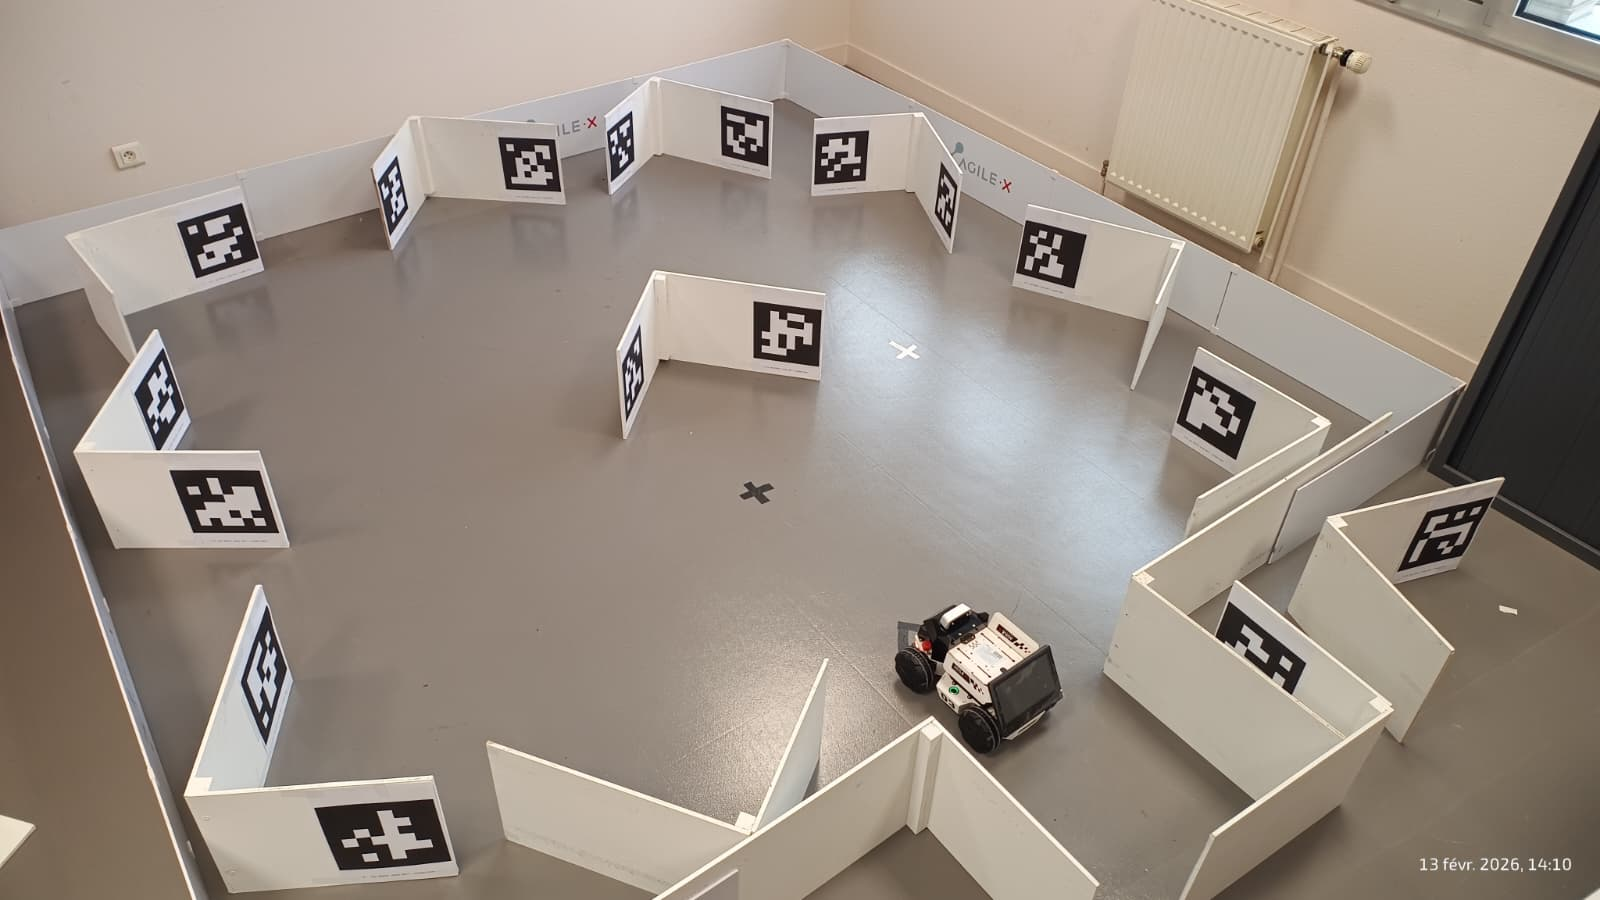
\includegraphics[width=0.96\linewidth,height=0.35\textheight,keepaspectratio]{../Report/Images/limo_real_environment.png}\\[-0.4mm]
      {\tiny Real setup with LIMO and AprilTags}
    \end{column}
    \begin{column}{0.5\textwidth}
      \centering
      \only<2->{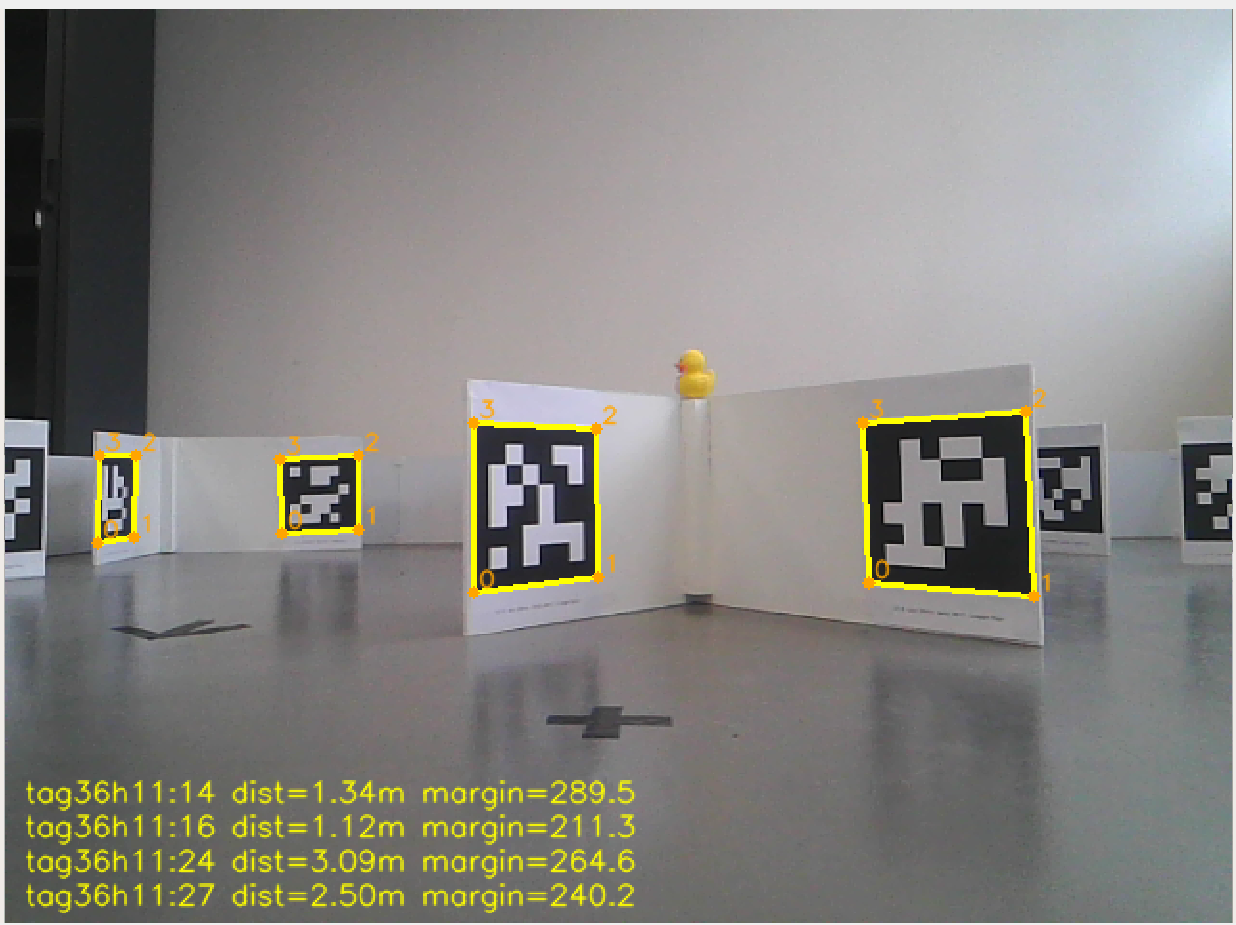
\includegraphics[width=0.96\linewidth,height=0.35\textheight,keepaspectratio]{assets/detections.png}\\[-0.4mm]}
      \only<2->{\tiny Detection's frame }
    \end{column}
  \end{columns}
\end{outlinecard}

\vspace{-0.12cm}
\begin{outlinecard}[Setup Flow]
  \centering
  \begin{tikzpicture}[x=1cm,y=1cm,>=Latex]
    % steps
    \node<1->[draw=NavyBlue!70, fill=white, rounded corners=1.2pt, line width=0.75pt,
      minimum width=2.70cm, minimum height=0.86cm, align=center] (s1) at (1.55,0.90)
      {\scriptsize\textbf{1) Drive}};
    \node<2->[draw=NavyBlue!70, fill=white, rounded corners=1.2pt, line width=0.75pt,
      minimum width=2.70cm, minimum height=0.86cm, align=center] (s2) at (4.65,0.90)
      {\scriptsize\textbf{2) Record}};
    \node<3->[draw=NavyBlue!70, fill=white, rounded corners=1.2pt, line width=0.75pt,
      minimum width=2.70cm, minimum height=0.86cm, align=center] (s3) at (7.75,0.90)
      {\scriptsize\textbf{3) Optimize}};
    \node<4->[draw=NavyBlue!70, fill=white, rounded corners=1.2pt, line width=0.75pt,
      minimum width=2.70cm, minimum height=0.86cm, align=center] (s4) at (10.85,0.90)
      {\scriptsize\textbf{4) Export}};

    % active marker
    \fill<1>[AccentGold] ($(s1.north west)+(0.04,-0.04)$) rectangle ($(s1.north west)+(0.15,-0.33)$);
    \fill<2>[AccentGold] ($(s2.north west)+(0.04,-0.04)$) rectangle ($(s2.north west)+(0.15,-0.33)$);
    \fill<3>[AccentGold] ($(s3.north west)+(0.04,-0.04)$) rectangle ($(s3.north west)+(0.15,-0.33)$);
    \fill<4>[AccentGold] ($(s4.north west)+(0.04,-0.04)$) rectangle ($(s4.north west)+(0.15,-0.33)$);

    % arrows
    \draw<2->[NavyBlue!60, line width=0.8pt, -{Latex[length=1.8mm,width=1.3mm]}] (2.9,0.90) -- (3.3,0.90);
    \draw<3->[NavyBlue!60, line width=0.8pt, -{Latex[length=1.8mm,width=1.3mm]}] (6.0,0.90) -- (6.4,0.90);
    \draw<4->[NavyBlue!60, line width=0.8pt, -{Latex[length=1.8mm,width=1.3mm]}] (9.1,0.90) -- (9.5,0.90);

    % visual icons above each step
    % 1) joystick
    \begin{scope}[visible on=<1->]
      \fill[AccentBlue!20] (1.55,1.30) circle (0.16);
      \draw[NavyBlue, line width=0.7pt] (1.55,1.30) circle (0.16);
      \node[text=NavyBlue, font=\scriptsize] at (1.55,1.30) {\faGamepad};
    \end{scope}

    % 2) rosbag database
    \begin{scope}[visible on=<2->]
      \fill[AccentBlue!20] (4.65,1.30) circle (0.16);
      \draw[NavyBlue, line width=0.7pt] (4.65,1.30) circle (0.16);
      \node[text=NavyBlue, font=\scriptsize] at (4.65,1.30) {\faDatabase};
    \end{scope}

    % 3) optimize
    \begin{scope}[visible on=<3->]
      \fill[AccentBlue!20] (7.75,1.30) circle (0.16);
      \draw[NavyBlue, line width=0.7pt] (7.75,1.30) circle (0.16);
      \node[text=NavyBlue, font=\scriptsize] at (7.75,1.30) {\faCogs};
    \end{scope}

    % 4) export file
    \begin{scope}[visible on=<4->]
      \fill[AccentBlue!20] (10.85,1.30) circle (0.16);
      \draw[NavyBlue, line width=0.7pt] (10.85,1.30) circle (0.16);
      \node[text=NavyBlue, font=\scriptsize] at (10.85,1.30) {\faFile};
    \end{scope}
  \end{tikzpicture}
\end{outlinecard}
